\section{Health Outcomes in the Future Adult Model (FAM)} \label{appendix:health}

\noindent \textbf{[JJH: The last battle zone!]}

\noindent \textbf{[JLG: I have reworked this version, based on your comments and on my conversations with Bryan and Duncan. I have gotten rid of a lot of the extensive verbal introduction and many other verbal details that now have become schematic and clear with the presentation of what we estimate and the big tables that I generated.]}

Our methodology to forecast and monetize health outcomes is a modified version of Section~\ref{section:cbamethodology}. When studying labor income, a first-order autoregressive model is a helpful device to simplify a complex reality and produce forecasts. As it turns out, in the paper we find that model to perform well under a variety of testable implications. 

When studying health, a modified version is needed because there is abundant state interdependency in health outcomes. We use a dynamic microsimulation model (the Future Adult Model - FAM) as laboratory to estimate health-state occupancy probabilities and to predict other health and economic outcomes. With this in hand, we forecast the health trajectories of the ABC/CARE individuals. In Section~\ref{section:cbamethodology}, we initialize the forecast of labor income using labor income at age 21. In this appendix, we use a ABC/CARE rich age-30 interview and a health follow-up conducted when the subjects were in their mid-30s to initialize the forecast of the health trajectory. We then monetize health outcomes using quality-adjusted life years and medical costs.\footnote{This microsimulation model is an extension of the model used by \citet{Prados_etal_2015_How-Much-Can-Education}; the technical details are described in \citet{Goldman_etal_2015_Future-Adult-Model}. Both models are related to the Future Elderly Model (FEM), which is a microsimulation tool originally developed to examine the health and health care costs among the elderly Medicare population \citep{Goldman_etal_2004_RAND-Report_Health-Status-Elderly}. It has been used extensively to assess health and disease prevention scenarios: FEM has been used to assess the future costs of disease, the benefits of preventing disease among older population, the consequences of new medical technologies, trends in disability, and the fiscal consequences of worsening population health (see \citet{Goldman_etal_2004_RAND-Report_Health-Status-Elderly}, \citet{Lakdawalla_etal_2004_Health-and-Cost}, \citet{Goldman_etal_2005_HA}, and \citet{Zissimopoulos_etal_2014_Delaying-Alzheimers}). The main differences with FEM are that the model we use starts with cohorts of individuals at age 30 instead of 50, and that it simulates more outcomes than FEM, because they are important to explain health outcomes and medical expenditure at younger ages, like evolution of partnership and marital status, work status, and family size.}

\noindent Before providing formal details, we summarize the data sets used, as well as variable construction and imputation assumptions.

\subsection{Data Sources} \label{section:data}
\noindent FAM uses data from ABC/CARE follow-up surveys to build the initial state of the cohort. 
The transition model parameters are estimated from the 1997 to 2013 waves of the Panel Study of Income Dynamics (PSID). 
We supplement the PSID with data from the Health and Retirement Study (HRS). We use the National Health and Nutrition Examination Survey (NHANES) 
to account for differences between measured and self-reported BMI.
To estimate medical care costs associated with health conditions, we use the Medical Expenditures Panel Survey (MEPS) and the Medicare Current Beneficiaries Survey (MCBS). \\


\subsubsection{PSID}
\label{section:data_psid}
%The Panel Survey of Income Dynamics (PSID) is a longitudinal household survey containing between 5,000 and 8,500 families in each wave, which began yearly in 1968 and is fielded biennially since 1996. When appropriately weighted, the PSID is designed to be representative of U.S. households. The PSID provides extensive information concerning demographics, economic outcomes, health care access, health outcomes, and health behaviors (such as smoking history, alcohol consumption, and exercise habits). Health outcome variables include diagnosis of diabetes, heart disease, hypertension, lung disease, cancer, etc. 

\noindent The Panel Study  of Income Dynamics (PSID) provides extensive information concerning demographics, economic outcomes, health care access, health outcomes, and health behaviors (such as smoking history, alcohol consumption, and exercise habits). Health outcome variables include diagnosis of diabetes, heart disease, hypertension, lung disease, and cancer, among others.\\

\noindent We estimate the transition models using waves from 1997 to 2013. We create a dataset of respondents who have formed their own households, either
as single heads of households, cohabiting partners, or married partners.  These heads, wives, and husbands respond to the richest
set of PSID questions, including the health questions that are critical for our purposes. We use all respondents aged 25 and older.\footnote{While we use the full sample, we explored using a few different subsamples to better adapt to the demographics of the ABC/CARE subjects.}  
The length of the PSID is a significant advantage, because we can include past health behaviors as explanatory variables for current health outcomes. This dataset provides adequate sample sizes to explore health outcomes of specific groups. 
PSID does not follow individuals who are institutionalized in nursing homes or other long-term care facilities. To overcome this weakness, we pool the PSID sample with the HRS sample when
estimating mortality models. \\

\subsubsection{HRS}

\noindent The Health and Retirement Study (HRS) is a longitudinal panel that surveys a nationally representative sample of individuals over the age of 50 and their spouses every two years.  When appropriately weighted, the HRS in 2010 is representative of U.S. households 
where at least one member is at least 51 years old.
This study collects in-depth information about income, work, health, and medical expenditures. In our model, waves from 1998 to 2012 are pooled with the PSID for estimation of mortality and 
widowhood models. The HRS data
are harmonized to the PSID for all relevant variables. Because PSID does not follow respondents into nursing homes, we also use the HRS to estimate the model for nursing home residency.  We use all cohorts in the dataset created by RAND (RAND HRS, version O) as the basis 
for our analysis. \\

\subsubsection{MCBS}
\noindent The Medicare Current Beneficiary Survey (MCBS) is a nationally representative sample of aged, disabled, 
and institutionalized Medicare beneficiaries.  The MCBS attempts to interview each respondent twelve 
times over three years, regardless of whether he or she resides in the community, a facility, or 
transitions between community and facility settings. The disabled (under 65 years of age) and 
very elderly (85 years of age or older) are over-sampled. The first round of interviewing was conducted 
in 1991. Originally, the survey was a longitudinal sample with periodic supplements and indefinite 
periods of participation. In 1994, the MCBS switched to a rotating panel design with limited periods 
of participation. Each fall, a new panel is introduced, with a target sample size of 12,000 respondents. Each summer, a panel is retired. Institutionalized respondents are interviewed by proxy.  The MCBS 
contains comprehensive self-reported information on the health status, health care use and 
expenditures, health insurance coverage, and socioeconomic and demographic characteristics of the 
entire spectrum of Medicare beneficiaries.  Medicare claims data for beneficiaries enrolled in 
fee-for-service plans are also used to provide more accurate information on health care use and 
expenditures.  MCBS data from 2007 to 2010 are used for estimating medical costs and enrollment models. \\

\subsubsection{MEPS}
\noindent The Medical Expenditure Panel Survey (MEPS), which began in 1996, is a set of large-scale surveys of families and individuals, their medical providers, and employers across the U.S. The Household Component (HC) of the MEPS provides data from 
individual households and their members, which is supplemented by data from their medical providers. 
The HC collects data from a representative subsample of households drawn from the 
previous year's National Health Interview Survey (NHIS). Since NHIS does not include the 
institutionalized population, neither does MEPS; this implies that we can only use the MEPS to 
estimate medical costs for the non-elderly (ages 25--64) population. Information collected during household 
interviews include: demographic characteristics, health conditions, health status, use of medical 
services, sources of medical payments, and body weight and height. Each year the household survey 
includes approximately 12,000 households, or 34,000 individuals. Sample size for those aged 25-64 is 
about 15,800 in each year.  MEPS has comparable measures of socioeconomic status as those in PSID, 
including age, race and ethnicity, educational attainment, census region, and marital status.  We estimate medical expenditure 
and utilization using data from 2008 to 2010. We use waves from 2001 to 2003 to estimate models of quality-adjusted life years (QALYs), due to availability of EQ-5D instrument in these waves.\footnote{Section \ref{section:FAM_models} explains the estimation of the QALY model.} \\


\subsubsection{NHANES}
\noindent 
The National Health and Nutrition Examination Survey (NHANES) targets a nationally representative sample of approximately 5,000 individuals in each year since 1999.  The data collected includes responses to interview questions about demographics, disease conditions, height, and weight, as well as physical measurement of BMI.  We use NHANES years 2002 to 2010 to estimate a model for imputing measured BMI from self-reported BMI.  The methodology is described in Section \ref{section:FAM_ABC_impute}.

\subsubsection{ABC/CARE}
\noindent FAM uses ABC/CARE data to initialize the state of each ABC/CARE subject when they enter into the simulation.  
These data are taken from the the parental interviews at various subject ages from birth to age 21; age-30 subject interview; and mid-30s biomedical survey.  
The goal is to have each subject's initial state in the simulation match their status at the age-30 subject interview. However, because several key FAM inputs are not available at the age-30 interview, we use PSID or ABC/CARE surveys corresponding to other ages to impute missing elements. These imputations are discussed in Section \ref{section:FAM_ABC_impute}. \\

% \todo we could add a table of all the FAM input variables (rows) and three columns, as-is, rule imputed, model imputed, with checkmarks to indicate how the data were derived

\subsection{Methods and Analysis}

\subsubsection{ABC and CARE Data Assumptions and Imputations}
\label{section:FAM_ABC_impute}

% \todo would be nice to have a table that summarizes imputed variables at age 30, imputation method, and number of missing subjects

\noindent Marital status transitions and childbearing in FAM are affected by the subject's mother's education level. The ABC and CARE age-30 subject interview did not ask about mother's education, but the ABC age-21 parent interview did.
For ABC subjects, we assume that each subject's mother had the same education level at the age-30 subject interview as what was reported in the age-21 parent interview. For CARE subjects, we impute mother's education from an ordered Probit model using race, ethnicity, education, disease conditions, employment status, presence of a health-related work limitation, and a self-report of whether or not the subject was ``poor'' as a child.  The model is estimated using age 30 to 31 PSID subjects.  Each of the model covariate values are taken from the CARE age 30 interview. At the beginning of each simulation repetition, an education level is randomly drawn from the probability distribution for each CARE subject and assigned to be the mother's education level.  \\

\noindent Many FAM transition models depend on a three-level measure of parents' economic status when the subject was a child.
This is based on the PSID question: ``Were your parents poor when you were growing up, pretty well off, or what?''
The three possible responses are ``poor,'' ``average''/``it varied'', or ``pretty well off.''
This question is not included in the ABC or CARE interviews, but because preliminary eligibility for the program focused on children from high-risk backgrounds, based on socioeconomic factors, the value of this variable is set to ``poor'' (when growing up) for all ABC and CARE subjects. \\

\noindent All FAM transition models depend on demographics of the subject, including whether or not the subject is Hispanic.
This information is not available in the ABC or CARE data, but it is assumed that none of the ABC or CARE subjects are Hispanic.\footnote{Census data on Hispanics in North Carolina were not available for 1970 and 1980, but Hispanic migration into this state is more recent than in other regions, and as late as 1990, only 2\% of the North Carolina poor were Hispanic \citep{Johnson_2003_Changing-Poverty}.} \\

\noindent Most FAM models depend on smoking status. Employment status affects FAM transitions in marital status, childbearing, claiming of disability insurance (DI) and supplemental security income (SSI), and type of health insurance.
One male in the ABC control group was missing smoking status and, although known to be not working, was also missing specific employment status (unemployed or out of the labor force).
 We use a multinomial logit model to jointly estimate the probability of each combined smoking and employment category among 25- to 35-year-olds in the PSID who were not working. At the beginning of each simulation repetition, we use a Monte Carlo random draw generated from this distribution to assign this subject's smoking and employment statuses. This same subject is also missing information about binge drinking.  A separate binary Probit binge drinking model was estimated using the age 25--35 PSID data. A Monte Carlo random draw is taken according the Probit probability to predict binge drinking behavior at the beginning of the simulation. \\
 
\noindent BMI affects FAM transitions in health, functional status, employment, and smoking.
The FAM transition models are estimated with BMI computed from self-reported height and weight in the PSID.
The only BMI data in ABC and CARE come from height and weight measured during the health interview. This interview took place at roughly age 30 for CARE subjects, and at age 34 for ABC subjects.
This poses two challenges.
First, self-reported BMI can be biased by factors such as actual height and weight, gender, and race.\footnote{\citet{Cawley_2004_JHR}.}
Second, it is possible that BMI could increase or decrease systematically in the years between the age-30 subject interview and the age-34 health interview. \\

\noindent To address the first BMI imputation challenge, we used a variation on the method of \citet*{Courtemanche_etal_2015_Adjusting-Body-Mass} to impute measured BMI in the PSID.
While the method in \citet{Courtemanche_etal_2015_Adjusting-Body-Mass} works with height and weight, we apply the specification to directly model BMI. Using respondents aged 30 to 40 in the 2002-2010 NHANES waves, we predict measured BMI from percentile ranks of self-reported BMI using the model specification in \citet{Courtemanche_etal_2015_Adjusting-Body-Mass}. Three variations 
on the spline interactions of \citet{Courtemanche_etal_2015_Adjusting-Body-Mass} were also considered.  After estimating this model using NHANES data, covariate values from the PSID 
age 30--34 data in years 2002--2013 were used to impute measured BMI values for PSID respondents. A Kolmogorov-Sminov (K-S) test and a visual inspection of smoothed histograms were used to compare the distribution of PSID imputed values to the distribution of observed values in the NHANES estimation sample.  The model specification selected for imputation had the smallest K-S distance between the two distributions.  The smoothed histogram of the distributions for the entire samples and the black subgroup in each data set appeared reasonably close.  \\

\noindent After imputing values of measured BMI for PSID respondents age 30--34, we turned to the second problem: accounting for systematic trends in BMI from the age 30 interview to the health interview.  The goal was to have a model that could map from measured BMI at the health interview around age 34 to self-reported BMI at the age 30 interview.  Employing the longitudinal structure of PSID, we matched each respondent's first interview between age 30--32 with their imputed measured BMI at between ages 33--40.  We then estimated a model using self-reported BMI between ages 30--32 as the response variable and imputed measured BMI at ages 33--40, the age when BMI is measured, along with other variables observed at age 30 as explanatory variables. This imputation model was applied to any ABC or CARE subject who has their health interview at least one year after their age 30 interview.\\

\noindent For ABC and CARE subjects who have their health interview within one year of the age 30 interview, we assumed that any systematic time trends in BMI are too small to have any practical significance.  However, we still needed to convert the imputed measured BMI to a self-reported value for compatibility with other transition models estimated in PSID.  This model was estimated on ages 30--32 in the PSID and uses covariates from the age 30 interview along with imputed measured BMI to predict self-reported BMI. \\

\noindent At the beginning of each simulation repetition, we chose the appropriate model to impute self-reported BMI for each ABC or CARE subject based on the time between their age 30 interview and their health interview. Their expected BMI was estimated from this model. A Monte Carlo Normal random draw was generated using the subject's expected BMI and the estimated variance from the model. This Monte Carlo draw was then assigned to be the subject's initial self-reported BMI in the simulation. Using BMI from the health interview limited the ABC and CARE subjects simulated in FAM to only those who had height and weight measured in the health interview. \\

\noindent Subjects' health insurance coverage affects their medical costs.
FAM uses three categories of health insurance: none, public only, and some private.
Five ABC subjects and three CARE subjects were missing health insurance status.
Three cases were logically imputed by assuming that subjects have no health insurance if they do not know their insurance status and either go to an emergency room or community health clinic or do not go anywhere when they need health care.
In order to impute the insurance category for the remaining five cases, we use age 25--35 PSID data to estimate a Probit model for whether or not a subject had insurance.
The predictors were gender, earnings, marital status, self-reported health, employment status, and whether or not the subject had any biological children.
We use this model to compute the probability of having insurance at the start of the simulation (at the age-30 interview).
Then, we generate a Monte Carlo binary random variate according to this probability.
If the outcome is positive, the subject is assigned to have some private insurance. \\

\noindent FAM uses six Activities of Daily Living (ADLs) about which there is data in PSID: walking, dressing, eating, bathing or showering, getting in and out of bed or a chair, and using the toilet, including getting to the toilet.
FAM simulates the number of these ADLs in which the subject has difficulty.
ADL difficulties predict FAM transitions in benefits claiming, mortality, employment status, insurance category, and nursing home residency.
FAM also transitions the count of difficulties among six Instrumental Activities of Daily Living (IADLs) from PSID: preparing one's own meals; shopping for personal toilet items or medicines; managing one's own money, such as keeping track of expenses or paying bills; using the phone; doing heavy housework, like scrubbing floors or washing windows; and doing light housework, like doing dishes, straightening up, or light housecleaning.
Both ADLs and IADLs are components of FAM's model for quality-adjusted life years (QALYs).
The ABC and CARE age-30 subject interview does not ask about ADLs or IADLs, but it does ask if the subject has a physical or nervous condition that keeps them from working.
PSID respondents are also asked this question.
We create an imputation model for each of these two measures using an ordered Probit model estimated on PSID respondents aged 25 to 35.
We use these models to compute the probabilities for each number of ADLs and IADLs. At the start of the the simulation, we generate Monte Carlo random draws according to these probabilities and use them to assign the corresponding counts. \\

\noindent When a subject claims DI benefits, it affects their FAM transitions in employment status, insurance category, and Medicare enrollment.
DI claiming also affects medical costs.
SSI claiming affects FAM transitions in employment status.
Lastly, claiming Social Security retirement benefits affects FAM transitions in employment status and insurance category.
The ABC age-30 subject interview has a single yes/no question about claiming which asks: ``Currently are you receiving income from workman's compensation, disability, or Social Security benefits including Supplemental Security Income?'' CARE asks a similar question. The PSID has separate questions for each benefit type. We use a multinomial logit model to estimate the joint probability of each combination of DI and SSI claiming. The estimation uses PSID respondents aged 25 to 35 who were claiming at least one of the following benefits: workman's compensation, DI, or SSI. A Monte Carlo random draw generated from this distribution is used to assign each ABC and CARE subject's DI- and SSI-claiming status at the start of the simulation. One ABC subject is missing data about whether or not they were claiming and was assumed to not be claiming any benefits.\\

\noindent As discussed in Section \ref{section:FAM_models}, FAM uses different models to estimate medical costs depending on whether or not a subject is Medicare-eligible. Subjects can enroll in Medicare before the age of 65 if they are claiming DI. The cost estimates for Medicare-eligible subjects depend on the subjects' current disease status at the age-30 interview and their disease status two years prior to the interview. Unfortunately, ABC and CARE do not have disease data two years before the age-30 interview. It is assumed that all subjects did not have their disease conditions in the previous period. In other words, for any subjects who reported a disease condition in the age-30 interview, their costs in the first simulation time step is estimated as if it were their incident year of the disease. Section \ref{section:FAM_models} describes the implications of this assumption. \\

% \todo capital income -- imputed, but not used as an outcome

% \todo we will include health conditions at age 30 in covariates of health dynamics

% \todo health as a child -- are we going to ignore this?

% \todo summarize disease conditions at age 30? -- important point: one female in control group has cancer at age 30

\subsubsection{FAM Models and Estimation}
\label{section:FAM_models}

\noindent We develop models to estimate the determinants of transitions between health outcomes, labor market outcomes, educational attainment, and family formation, for individuals aged 25 and older.
Additionally, we estimate transition probabilities by gender, race and ethnicity, and educational attainment as a function of individual characteristics (see below).
Each transition model includes a subset of variables and relevant interactions from the following list: age, gender, race and ethnicity, education, parents' education, self-reported body mass index (BMI), smoking history, physical activity, binge drinking, lagged health conditions, asthma diagnosis before age 30, number of biological children, past earnings and work status, partnership status (single, cohabiting, married, separated/divorced, or widowed), disability status, and health insurance status.
We consider three racial and ethnic groups (black non-Hispanic, white non-Hispanic, and Hispanic), and four educational groups (less than high school degree; high school graduate, including some college or associate's degree; college; and more than college). \\

\noindent The health transition models estimate the probability that a person transitions between health states, e.g. obesity or heart disease, as a function of current health status, demographic characteristics (including race, gender, age, and education), and risk factors (including weight, smoking status, physical activity, asthma, and number of births if female for BMI transitions), enabling us to age the cohorts. This mechanism to model health transitions accounts for the fact that certain health conditions increase the likelihood of comorbidities.
We estimate a transition model for each of the following health conditions: heart disease, blood pressure, stroke, lung disease, diabetes, and cancer. Each disease model includes gender, race and ethnicity, and educational group as covariates.
We select conditions that are prevalent in the U.S. and are characterized by significant disparities in outcomes across education, race and ethnicity, and income. 
The reason for this is that the incidence and progression of these conditions can potentially be reduced by preventive services, education policies, and modifications in health behaviors. 
These chronic conditions are treated as absorbing states, i.e., once the individual transitions into a chronic condition, the condition persists until death. \\

\noindent Additionally, we allow individuals to transition in and out of risk factors, such as smoking, binge drinking, and BMI. These transitions are estimated as a function of demographics, past health, and risk factors.
In the estimation, changes in risk behaviors alter future health outcomes and risk factors (e.g., smoking cessation may impact changes in BMI, and continuing smoking may affect incidence of lung disease). We also transition mental health, approximated by the Kessler mental distress scale, which is one of the predictors of the medical costs models.
\\

%describe models of ADLs IADLs estimation

\noindent Because the PSID sample covers a broad age range, it is smaller than the HRS sample at older ages where mortality becomes more likely. Also, the PSID does not follow respondents into nursing homes.
Therefore, the FAM mortality model is estimated using a pooled PSID and HRS sample.
The mortality model includes these covariates: age, gender, race and ethnicity, education, disease conditions, ADL count, binge drinking and current smoking status.
Similarly, a partner mortality model is estimated from the pooled PSID and HRS data for transitions into widowhood.
The covariates in the partner mortality model are age, gender, race and ethnicity, and education.
These covariates are characteristics of the respondents, not the partners who are facing mortality (FAM does not simulate the characteristics of partners). \\

\noindent Since the PSID does not follow respondents into nursing homes, the model for nursing home residency is estimated using only HRS data. It includes these covariates: age, gender, race and ethnicity, education, disease conditions, ADL and IADL counts, and widowhood. \\

\noindent The marriage transition model estimates transitions between partnership status (we distinguish between single, cohabiting, and married).
The model is a function of demographics, past employment status, earnings, mother's education and number of children.
There are also childbearing models that estimate new births for each gender.
Childbearing is modeled as an ordered probit model that is a function of past health and birth history, demographics, education, past work status, and past partnership status. \\

\noindent The employment status model estimates the probability that a person transitions into different employment states (unemployed, out of the labor force, working part-time, or working full-time).  This transition is a function of demographics, marital or partnership status, education, health status and behaviors, past earnings and benefits claiming. \\

% \todo health insurance category -- once it is implemented

% \todo SSI/DI/SS benefits claiming -- once it is implemented

\noindent The combination of transition models allows us to address the aspects of the life-cycle that are most relevant for the proposed analysis. To complete the analysis, there are also models to estimate QALYs, medical expenditure, and Social Security participation. \\

\noindent We compute a QALY model based on the EQ-5D instrument, a widely-used, health-related
quality-of-life (HRQoL) measure. %\footnote{Section \ref{sec:model_development_qalys_hrqol} gives some background on HRQoL measures.}
The scoring system for EQ-5D was first developed using a U.K. sample.\footnote{\citet{Dolan_1997_Modeling_MC}.} Later, a scoring system based on
a U.S. sample was generated.\footnote{\citet{Shaw_etal_2005_EQ5D_MC}.} The PSID does not ask the appropriate questions for computing EQ-5D, but the MEPS does. \\

% review this:
\noindent We map EQ-5D scores from the MEPS onto the PSID data using common measures between the MEPS and PSID.\footnote{The main variables in this mapping are self-reported health and requiring help with ADLs.} We then predict the EQ-5D scores for all PSID members running a linear regression using the variables that are transitioned in FAM (including ADL counts, IADL counts, and diseases). The microsimulation uses this linear regression to compute QALYs. \\
%
%We use a crosswalk from MEPS to compute EQ-5D scores for PSID respondents.\footnote{Section \ref{sec:model_development_qalys_eq5d}
%describes EQ-5D in MEPS. Details of the crosswalk model development are given
%in \ref{sec:model_development_qalys_crosswalk}.}.
%The FAM has a more limited specification of functional status than what is available in the PSID. In order to predict
%HRQoL for the FAM simulation sample, we needed to build a bridge between the FAM-type functional status and the
%predicted EQ-5D score in the PSID. We use ordinary least squares to model the EQ-5D score predicted as a function of the six chronic conditions and the FAM-specification of functional status,
%%%


\noindent FAM has two versions of each medical cost model. For individuals who are not Medicare-eligible, the cost models are estimated from MEPS data.
Once an individual becomes Medicare-eligible, their costs are estimated from MCBS data. Both sets of models include the following covariates:
age, gender, race and ethnicity, education level, relationship status, disease conditions, and earnings.
The MEPS models also include type of health insurance as a covariate.
Because MCBS follows respondents for more than two years (the time step length in the FAM simulation), the FAM cost models for the Medicare-eligible population include covariates for the stage of each disease.
In the initial stage, a patient has a diagnosis in the current two-year period, but did not have the diagnosis in the previous two-year period.
Then, in the maintenance stage, a patient had a diagnosis in the previous two-year period and survives with the diagnosis in the current two-year period (all disease states are absorbing---it is impossible to transition out of a diagnosis).
Finally, in the terminal stage, a patient has a diagnosis and dies in the current two-year period.
The medical costs models tend to underestimate health care spending reported in the National Healthcare Expenditures Account (NHEA) data, due in part to underreporting of Medical costs in MEPS. \\

% Pasted from estimation in Technical Appendix:
\subsubsection{Transition Models}
\label{section:transition_models}

\noindent We denote
$j_{i,0}$ to be the first age at which subject $i$ is observed and $j_{i,T_i}$ the
last age at which he is observed. Hence, we observe outcomes at ages
$j_i = j_{i,0},\ldots,j_{i,T_i}$.
We first start with discrete outcomes which are absorbing states (e.g. disease
diagnostic, mortality, and benefit claiming). We record the hazard as $h_{i,j_i,m}=1$ if the
individual outcome $m$ has occurred as of age $j_i$. We assume the
individual-specific component of the hazard can be decomposed into time-invariant and time-variant parts. The time-invariant part is composed of the effect of
observed characteristics, $x_i$, that are constant over the entire life course and
initial conditions, $h_{i,j_0,-m}$, (where $-m$ denotes outcomes other than the outcome
$m$) that are determined before the first age in which each subject is observed. \\

%\footnote{Section \ref{sec:model_development_transition_model} explains why the $h_{i,j_0,-m}$ terms are included.}.
\noindent The time-variant part is the effect of previously diagnosed outcomes, $h_{i,j_i-1,-m}$,
on the hazard for $m$.\footnote{With some abuse of notation, $j_i-1$ denotes
the previous age at which the subject was observed.} We assume an index of
the form $z_{j_i,m} = x_i\beta_m + h_{i,j_i-1,-m} \gamma_m + h_{i,j_0,-m}\psi_m$. Hence, the
latent component of the hazard is modeled as
\begin{equation}
h^*_{i,j_i,m}= x_i\beta_m + h_{i,j_i-1,-m} \gamma_m + h_{i,j_0,-m}\psi_m + a_{m,j_i} + \varepsilon_{i,j_i,m},
\label{eqn:transition_hzd_latent}
\end{equation}
where $m = 1,\ldots,M$, $j_i = j_{i0},\ldots,j_{i,T_i}$, and $i=1,\ldots,N$.
The term $\varepsilon_{i,j_i,m}$ is a time-variant shock specific to age $j_i$.
We assume that this last shock is normally distributed and uncorrelated across
diseases. We approximate $a_{m,j_i}$ with an age spline with knots at ages 35, 45,
55, 65, and 75.
This simplification is made
for computational reasons since the joint estimation with unrestricted age fixed
effects for each condition would imply a large number of parameters. The
absorbing outcome, conditional on being at risk, is defined as
\begin{equation*}
h_{i,j_i,m} = \max\{I(h^*_{i,j_i,m} > 0), h_{i,j_i-1,m}\}.
%\label{eqn:transition_outcome}
\end{equation*}
The occurrence of mortality censors observation of other
outcomes in a current year. \\
% Mortality is recorded from exit interviews.

\noindent A number of restrictions are placed on the way feedback is allowed in the model. Our microsimulation model starts the health predictions at age 30, with the information on observed characteristics available at this age. We restrict it to the individuals for whom we have information from the health follow-up. This allows us to account for components that are crucial for predicting health outcomes, such as the body mass index (BMI). In sum, the models predict the probability of being in any of the states in the horizontal axis of Table~\ref{table:transition} at age $a+1$ based on the state at age $a$, which is described by the vertical axis of the table. The crosses indicate if the estimation of the probability of being in a state at age $a+1$ considers the relevant state at age $a$. Absorbing states are an exception. For example, heart disease at age $a$ does not enter in the estimation of transitions for heart disease at age $a+1$ because it is an absorbing state: once a person has heart disease, she carries it through the rest of her life. The same is true for chronic or permanent conditions such as hypertension, having a stroke, etc. \\

\begin{sidewaystable}[H]
\begin{threeparttable}
\caption{Health State Transitions, Age $a$ as Predictor of Age $a+1$}\label{table:transition}
\scriptsize
\begin{tabular}{l|cccccccccccccc} \toprule
\multicolumn{1}{c}{Age $a$} & \multicolumn{14}{c}{Age $a+1$} \\ \midrule
  & Heart & Hyper- & Stroke & Lung  & Diabetes & Cancer & Disability & Mortality & Smoking  & Obesity & Health  & DI  & SS  & SSI  \\
&  Disease & tension &  & Disease & & & & &  &  & Insurance & Claim & Claim & Claim \\
Heart Disease & & & $\times$& & & &$\times$ &$\times$ & $\times$           &       &  $\times$  & $\times$ & $\times$ & $\times$\\
Hypertension  &  $\times$& & $\times$ & & & &$\times$ &$\times$ &       &     & $\times$   & $\times$ & $\times$  & $\times$\\
Stroke           & & & & & & &$\times$ &$\times$ &             &      &   $\times$  & $\times$ & $\times$  & $\times$\\
Lung Disease & & & & & & &$\times$ &$\times$ & $\times$         &        &   $\times$  &$\times$  & $\times$  & $\times$\\
Diabetes       & $\times$ &$\times$  & $\times$   & & & &$\times$ &$\times$ & $\times$            &       &  $\times$    & $\times$& $\times$ & $\times$ \\
Cancer         & & & $\times$ &  & &   &$\times$ & $\times$&           &         &   $\times$  & $\times$ & $\times$  & $\times$\\
Disability     & & & & & & &$\times$ &$\times$ &         &      &     $\times$  & $\times$ & $\times$   & $\times$\\
\midrule
Smoking & $\times$& $\times$&$\times$ & $\times$& $\times$& $\times$&$\times$ &$\times$ & $\times$   &   &     $\times$  & $\times$ & $\times$   & $\times$\\
BMI & $\times$& $\times$&$\times$ & $\times$& $\times$& $\times$&$\times$ & & $\times$    &  $\times$ &     &  &   & \\
Physical Activ. & $\times$& $\times$&$\times$ & $\times$& $\times$& $\times$&$\times$ & & $\times$    &   &     &   &  & \\
Binge Drinking & & & & & & &  &$\times$ & $\times$    &      &      &   &     &  \\
\midrule
DI Claim      & & & & &  & & & &             &         & $\times$    & $\times$   & $\times$ & $\times$\\
SS Claim     & & & & & & & &           &         &     & $\times$ &  & & $\times$\\
SSI Claim   & & & & &&  & & &         &        &      & &   & $\times$\\ \bottomrule
\end{tabular}

{\flushleft\footnotesize
Note: This table illustrates how health outcomes at age $a$ predict health outcomes at age $a+1$. The crosses indicate if we use the age $a$ outcome to predict the age $a+1$ outcome. DI Claim: disability insurance claim; SS Claim: social security claim; DB Claim: disability benefits claim; SSI Claim: supplemental security income claim. The age $a$ states that do not predict themselves at age $a+1$ are absorbing states by construction.}
\end{threeparttable}
\end{sidewaystable}

%\begin{sidewaystable}[H]
%\begin{threeparttable}
%\footnotesize
%\caption{Restrictions on transition models} \label{table:transition}
%\scalebox{0.77}{
%\begin{tabular}{l*{17}{c}}
Value at time $T-1$ & \multicolumn{17}{c}{Outcome at time $T$}  \\
\hline
 					        & Heart      &              &            & Lung    &          &        &            &            & Smoking    &            & Health     &            &            &            & Nursing    & Work       &            \\
                  & disease    & Hypertension & Stroke     & disease & Diabetes & Cancer & Disability & Mortality  & status     & BMI        & Insurance  & DI Claim   & SS Claim   & SSI Claim  & Home       & Status     & Earnings   \\
Heart disease     &            &              & \checkmark &         &          &        & \checkmark & \checkmark & \checkmark &            & \checkmark & \checkmark & \checkmark & \checkmark & \checkmark & \checkmark & \checkmark \\
Blood pressure    & \checkmark &              & \checkmark &         &          &        & \checkmark & \checkmark &            &            & \checkmark & \checkmark & \checkmark & \checkmark & \checkmark & \checkmark & \checkmark \\
Stroke            &            &              &            &         &          &        & \checkmark & \checkmark &            &            & \checkmark & \checkmark & \checkmark & \checkmark & \checkmark & \checkmark & \checkmark \\
Lung disease      &            &              &            &         &          &        & \checkmark & \checkmark & \checkmark &            & \checkmark & \checkmark & \checkmark & \checkmark & \checkmark & \checkmark & \checkmark \\
Diabetes          & \checkmark & \checkmark   & \checkmark &         &          &        & \checkmark & \checkmark & \checkmark &            & \checkmark & \checkmark & \checkmark & \checkmark & \checkmark & \checkmark & \checkmark \\
Cancer            &            &              & \checkmark &         &          &        & \checkmark & \checkmark &            &            & \checkmark & \checkmark & \checkmark & \checkmark & \checkmark & \checkmark & \checkmark \\
Disability        &            &              &            &         &          &        & \checkmark & \checkmark &            &            & \checkmark & \checkmark & \checkmark & \checkmark & \checkmark & \checkmark & \checkmark \\
Claimed DI        &            &              &            &         &          &        &            &            &            &            & \checkmark & \checkmark & \checkmark & \checkmark &            & \checkmark & \checkmark \\
Claimed SS        &            &              &            &         &          &        &            &            &            &            & \checkmark &            &            & \checkmark &            & \checkmark & \checkmark \\
Claimed SSI       &            &              &            &         &          &        &            &            &            &            &            &            &            & \checkmark &            & \checkmark & \checkmark \\
Work              &            &              &            &         &          &        &            &            &            &            & \checkmark & \checkmark & \checkmark & \checkmark &            & \checkmark & \checkmark \\
Earnings          &            &              &            &         &          &        &            &            &            &            & \checkmark & \checkmark & \checkmark & \checkmark &            & \checkmark & \checkmark \\
Nursing home stay &            &              &            &         &          &        &            &            &            &            &            &            &            &            & \checkmark &            &         
\end{tabular}
%}
%\begin{tablenotes}
%\footnotesize
%\item Note: \checkmark indicates that an outcome at time $T-1$ is allowed in the transition model for an outcome at time $T$.
%\end{tablenotes}
%\end{threeparttable}
%\end{sidewaystable}


\noindent We have five other types of outcomes: \\
\begin{enumerate}
\item Binary outcomes that are not absorbing states, such as starting to smoke. We specify latent
indices as in Equation~\ref{eqn:transition_hzd_latent} for these outcomes as well but where
the lag-dependent outcome also appears as an independent variable. This allows for state-dependence.

\item Ordered outcomes, which are also modeled as in Equation~\ref{eqn:transition_hzd_latent} recognizing that the observation rule is
a function of unknown thresholds $\varsigma_m$. Similar to binary outcomes, we allow for state-dependence by including the lagged outcome
on the right-hand side.

\item Censored outcomes, such as capital income, are considered. For capital income,
there are a non-negligible number of observations with zero capital income. For these observations, we consider
two-part models where the latent variable is specified as in Equation~\ref{eqn:transition_hzd_latent} but models
probabilities only when censoring does not occur.

\item Continuous outcomes are modeled with linear models. An example continuous outcome is the
transitions in log(BMI). We allow for state-dependence by including the lagged outcome on the right-hand side.

\item Categorical models, but without an ordering, are considered. For example, an individual can transition
to being unemployed, out of the labor force, or working (either part- or full-time). In situations like this, we utilize
a multinomial logit model, including the lagged outcome on the right-hand side.

\end{enumerate}

\noindent In total, we have $M$ outcomes. The parameters
$\mathbf{\theta}_1 = \left(\left\{\beta_m, \gamma_m, \psi_m, \varsigma_m\right\}_{m=1}^M \right)$,
can be estimated by maximum likelihood. Given the normality distribution assumption on the
time-variant unobservable, the joint probability of all time-intervals until failure, right-censoring,
or death conditional on the initial conditions, $h_{i,j_0,-m}$, is the product of
normal univariate probabilities. Since these sequences, conditional on initial
conditions, are also independent across diseases, the joint
probability over all disease-specific sequences is simply the product of
those probabilities. \\

\noindent For a given subject observed from the initial age, $j_{i0}$, to the last age, $j_{T_i}$, the probability of the observed health history is
(omitting the conditioning on covariates for notational simplicity)
\begin{equation*}
	l^{-0}_i(\mathbf{\theta}; h_{i,j_{i0}}) = \left[\prod_{m=1}^{M-1} \prod_{j=j_{i1}}^{j_{T_i}} P_{ij,m}(\mathbf{\theta})^{(1-h_{ij-1,m})(1-h_{ij,M})} \right] \times \left[\prod_{j=j_{i1}}^{j_{T_i}} P_{ij,M}(\mathbf{\theta}) \right]
\end{equation*}
We use the ${-0}$ superscript to make explicit the conditioning on $\mathbf{h}_{i,j_{i0}} = (h_{i,j_{i0},0},\ldots,h_{i,j_{i0},M})'$. We have limited information on outcomes prior to this age.
The likelihood is a product of $M$ terms with the $m$th term containing only
$(\beta_m, \gamma_m, \psi_m, \varsigma_m)$. This allows the estimation
to be done separately for each outcome. \\

\paragraph{Further Details on Specific Transition Models}
\noindent This section describes the modeling strategy for particular outcomes. \\

\noindent \textbf{Employment Status}\\
\noindent Ultimately, we aim to simulate whether an individual is unemployed, out of the labor force, working part-time, or working full-time at
time $t$. We treat the estimation of this as a two-stage process. In the first stage, we predict whether the individual is unemployed, out of
the labor force, or working for pay using a multinomial logit model. Then, conditional on working for pay, we estimate if
the individual is working part- or full-time using a probit model. \\

\noindent \textbf{Relationship Status}\\
\noindent We are interested in three relationship statuses: single, cohabiting, and married. In each case, we treat the transition
from time $t$ to time $t+1$ as a two-stage process. In the first stage, we estimate if the individual will remain in his
current status. In the second stage, we estimate which of the two other states the individual will transition to, conditional
on leaving his current state. \\

\noindent \textbf{Childbearing}\\
\noindent We estimate the number of children born in two-year periods separately for females and males. We model this using an ordered probit with
three categories: no new births, one birth, and two births. Based on the PSID data, we found the exclusion of three or more
births in a two-year period to be appropriate. \\
%
%\subsubsection{Inverse Hyperbolic Sine Transformation}
%One problem fitting the wealth distribution is that it has a long right tail and some negative values. We use a
%generalization of the inverse hyperbolic sine transform (IHT) presented in \citet{mackinnon1990transforming}. First denote the variable of
%interest $y$. The hyperbolic sine transform is
%\begin{equation}
%y = \sinh(x) = \frac{\exp(x) - \exp(-x)}{2}
%\label{eqn:sinh_y}
%\end{equation}
%The inverse of the hyperbolic sine transform is
%\[
%x = \sinh^{-1}(y) = h(y) = \log(y + (1+y^2)^{1/2})
%\]
%Consider the inverse transformation. We can generalize such transformation, first allowing for a
%shape parameter $\theta$,
%\begin{equation}
%r(y) = h(\theta y)/\theta
%\label{eqn:generalized_ihs_shape}
%\end{equation}
%Such that we can specify the regression model as
%\begin{equation}
%r(y) = x\beta + \varepsilon, \varepsilon \sim \mathrm{N}(0, \sigma^2)
%\label{eqn:ihs_regression_model}
%\end{equation}
%A further generalization is to introduce a location parameter $\omega$ such that the new
%transformation becomes
%\begin{equation}
%g(y) = \frac{h(\theta(y+\omega)) - h(\theta\omega)}{\theta h'(\theta \omega)}
%\label{eqn:geralized_ihs_loc_scale}
%\end{equation}
%where $h'(a) = (1+a^2)^{-1/2}$.
%
%We specify (\ref{eqn:ihs_regression_model}) in terms of the transformation $g$. The shape parameters
%can be estimated from the concentrated likelihood for $\theta, \omega$. We can then
%retrieve $\beta, \sigma$ by standard OLS.
%
%Upon estimation, we can simulate
%\[
%\tilde{g} = x \hat{\beta} + \sigma \tilde{\eta}
%\]
%where $\eta$ is a standard normal draw. Given this draw, we can retransform using
%(\ref{eqn:geralized_ihs_loc_scale}) and (\ref{eqn:sinh_y})
%\begin{align*}
%&h(\theta(y+\omega)) = \theta h'(\theta\omega)\tilde{g} + h(\theta\omega)\\
%&\tilde{y} = \frac{\sinh\left[\theta h'(\theta\omega)\tilde{g} + h(\theta\omega)\right]-\theta\omega}{\theta}
%\end{align*}

% \todo link to transition_estimates.xls on box -- make link unique to the version of the appendix in make process
%The included estimates table (estimates\_FAM.xml) gives parameter estimates for the transition models.
% Ends estimation from Technical Appendix.



\subsubsection{FAM simulation}

\noindent A simulation of the model starts by loading the entering cohort, generated from the ABC and CARE data. Missing values are imputed with the imputation models described in section \ref{section:FAM_ABC_impute}.  To this entering cohort, the model applies the transition models for mortality, health, working status, family structure, wealth, and benefit claiming, estimated from PSID, with Monte Carlo decisions to calculate the new states of the population.
%The simulation is performed 5,000 times and the simulated distributions of key outcomes are summarized over repetitions. 
The simulated financial outcomes are in 2014 USD. \\


\noindent To match the biennial structure of the PSID data used to estimate the transition models, the simulation proceeds in two-year increments.\footnote{The end of each two-year step is designed to occur on July 1st to allow for easier matching with population forecasts from Social Security Administration (SSA).}
Once the new states have been determined, the cross-sectional models for medical costs and QALYs are applied.
Computation of medical costs includes the people who died to account for end-of-life costs.
The simulation ends when all simulated ABC and CARE subjects are deceased. Mortality is forced at age 120 if the simulated mortality model has not already predicted a subject's death. \\

\noindent Among the ABC and CARE subjects simulated in FAM, the years of completion of the age-30 interview range from 2003 to 2009.
FAM's two-year time step only allows the simulation of even or odd years.
For this reason, we ran the simulation twice---once for the ABC and CARE subjects entering in odd years and again for the ABC and CARE subjects entering in even years. \\

\noindent The simulation model takes as inputs assumptions regarding the normal retirement age, future improvements in mortality, and real medical cost growth.
% \DEL: interest rates assumptions apply to wealth -- not simulated
The normal retirement age is assumed to be 67 for all ABC and CARE subjects. \\

%% Wage growth has been turned off for this project
%\noindent Real wage growth projections are taken from the intermediate cost projections in Table VI.F6 of the 2009 Social Security Trustees Report\footnote{\citet{Trustees_2009_Annual-Report-Old-Age-Survivors}.} and then assumed to be 1.1\% annually in subsequent years.
%These wage-growth assumptions are plotted in Figure \ref{figure:nwi}. In each year of the simulation, the FAM earnings model predicts a subject's earnings in terms of 2009 USD.
%The earnings are then multiplied by the ratio of the current year index value to the 2009 index value in order to account for real wage growth since 2009. We then inflate our results to 2014 USD. \\

\noindent The FAM mortality model is assumed to represent mortality in 2009.
The estimated mortality probabilities are reduced in simulated future years to represent improvements in mortality from sources such as medical innovation that are not included in the model.
There are different adjustment factors for the populations under and over the age of 65.
The mortality reduction factors are taken from the intermediate cost mortality projections in the 2013 Social Security Trustee's Report.
The medical cost growth assumptions are derived from several underlying assumptions about growth in GDP and the labor force. \\

%% Not using NWI growth in this project
%\begin{figure}
%\caption{National Wage Index} \label{figure:nwi}
% \centering
%	 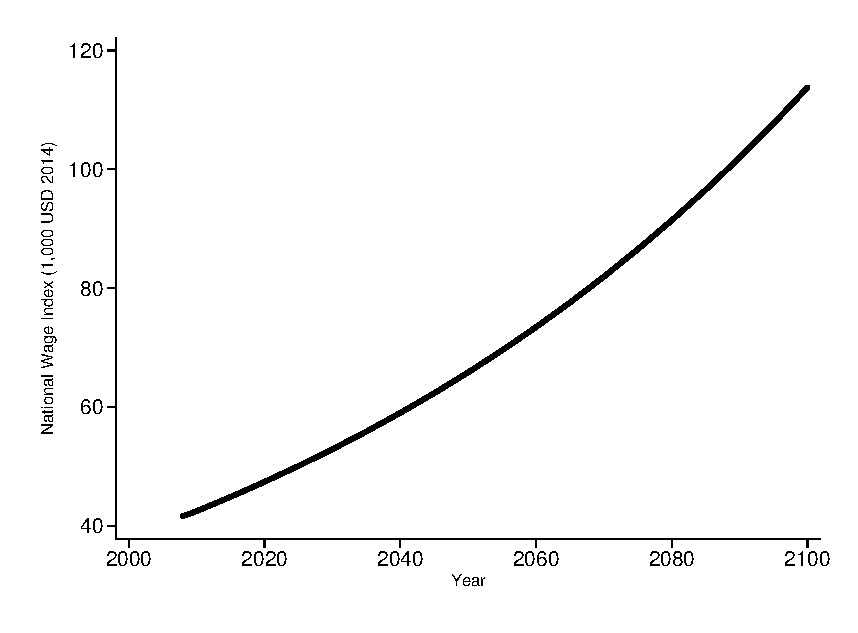
\includegraphics[height=3.5in]{AppOutput/Health/nwi.eps}
%\floatfoot{
%\footnotesize
%\noindent Note: Real wage growth projections are taken from Table VI.F6 in the 2009 Social Security Trustees Report \citep{Trustees_2009_Annual-Report-Old-Age-Survivors}. In years after the Trustees report projections, real wage growth is assumed to be 1.1\% annually.
%}
%\end{figure}

\noindent The real medical cost growth factor in each year is calculated by first finding the minimum of (i) the year-over-year GDP growth plus year-over-year excess medical cost growth or (ii) the Affordable Care Act cap on year-over-year medical cost growth. In order to obtain the medical cost adjustment factor for the current year of the simulation, FAM takes the cumulative product of the yearly growth factors since 2004 and then divides it by the relative growth in the labor force since 2004.\footnote{The medical cost growth assumptions come from Congressional Budget Office and SSA assumptions.
The year-over-year growth assumptions for medical costs are shown in Figure \ref{figure:medgrowth_yearly}.
The 2010-2019 GDP assumptions are based on CBO's analysis of the President's Budget, March 2009.
GDP assumptions for 2020-2100 are based on the 2008 OASDI Trustee's Report long-term projection of 2.1\% real GDP growth.} \\


\begin{figure}
\caption{Year-over-Year Excess Real Growth in Medical Costs} \label{figure:medgrowth_yearly}
 \centering
	 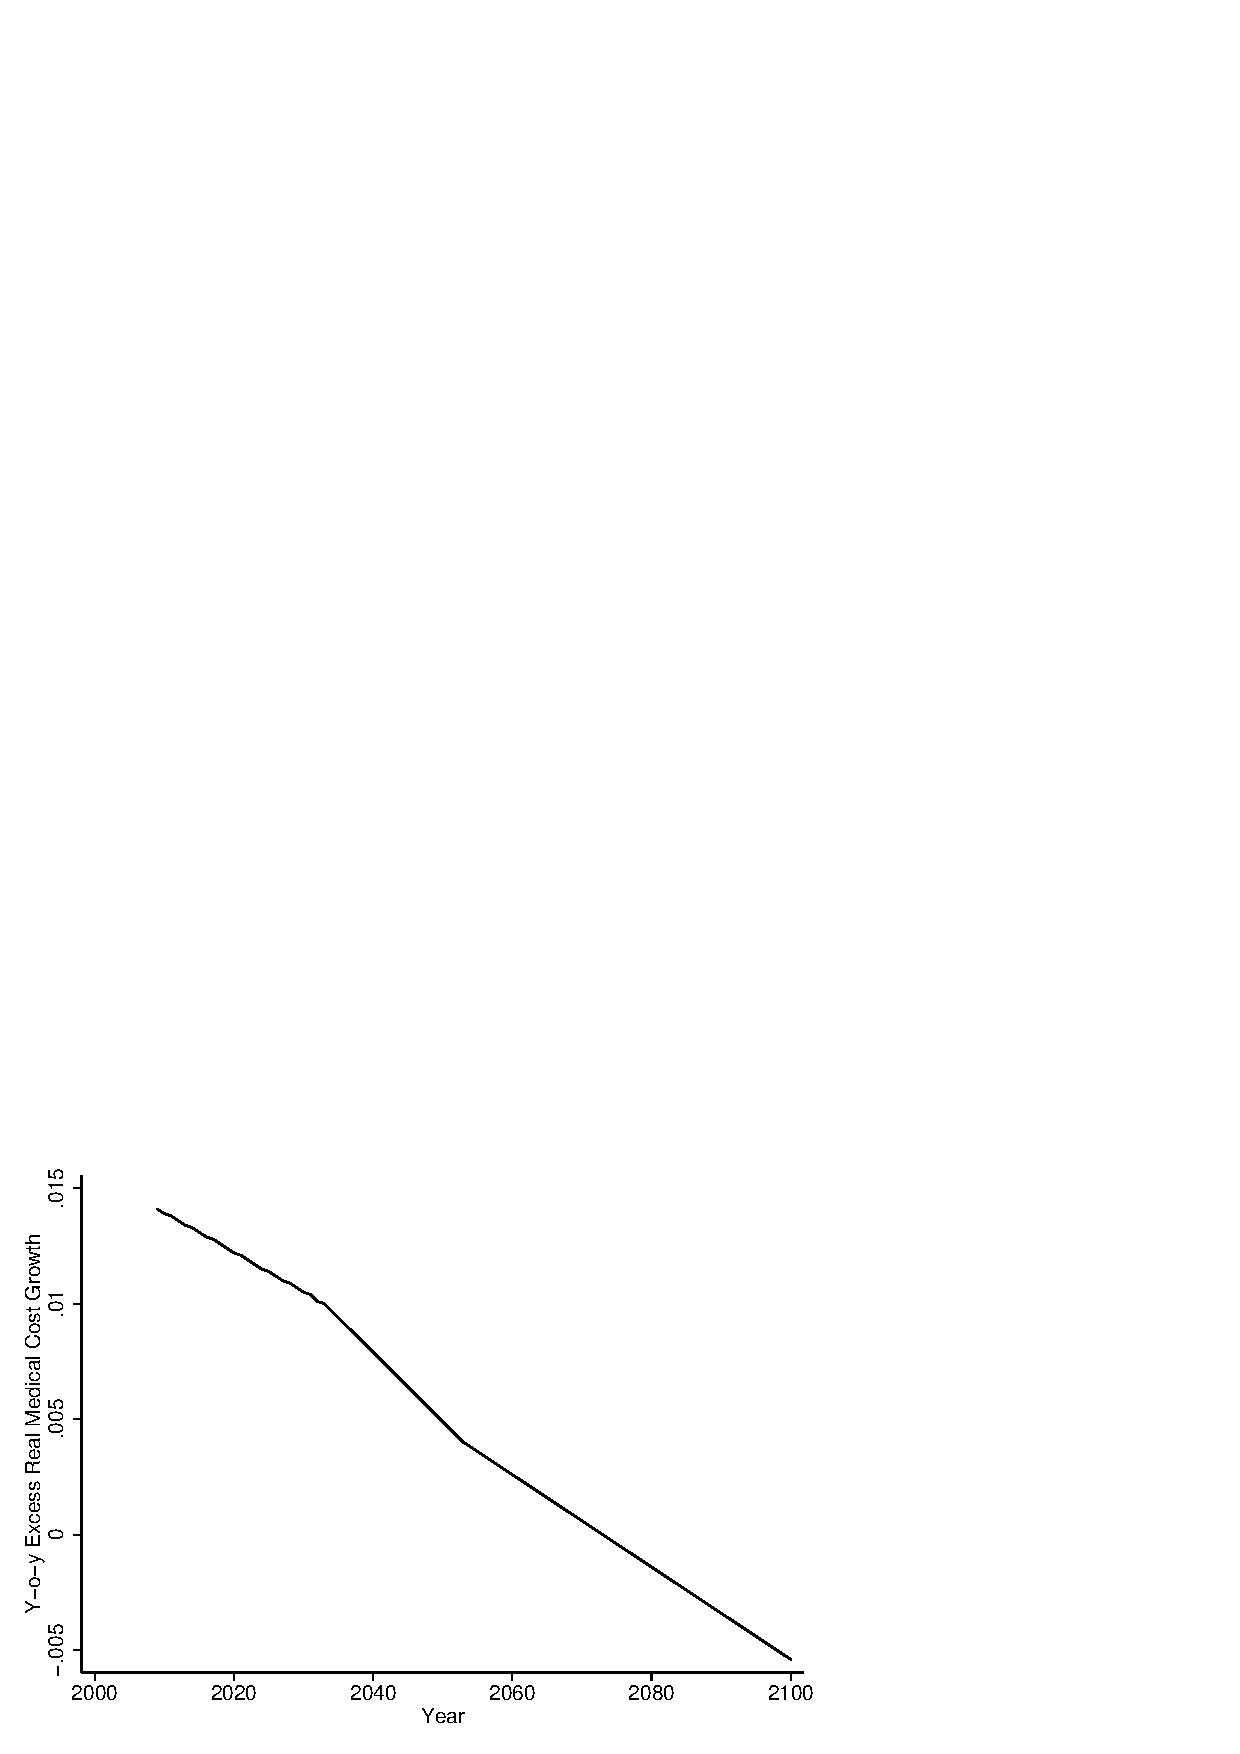
\includegraphics[height=3.5in]{AppOutput/Health/medgrowth_yearly}
\floatfoot{
\footnotesize
\noindent Sources: Congressional Budget Office, Social Security Administration.\\
\noindent Note: The year-over-year excess real medical cost growth over GDP is used to model medical cost growth in FAM.
}
\end{figure}

\subsubsection{Bootstrap Sampling Strategy}

\noindent The data sets used for estimating models in FAM are resampled in order to get estimates of sampling error in simulated outcomes.  PSID, HRS, MEPS, and MCBS all have complex survey designs that incorporate stratification and clustering.  In each of these data sets, the exact sampling strata and clusters are not publicly available, but approximations are included for the purpose of variance estimation.  The bootstrap methods in FAM were developed to implement the sampling strategy of \citet{McCarthy-Snowden_1985_Bootstrap}: randomly select $n_h-1$ sampling units with replacement from stratum $h$, where $n_h$ is the number of sampling units in stratum $h$. \\

\noindent PSID started with an initial sample of families in 1968.  Each generation of children from those families became sample members as they formed their own households.  The sample members present in the 1999--2013 PSID waves are used to estimate FAM models.   The PSID data used for estimation also includes a sample targeting immigrants that entered in 1997.  We randomly select one cluster from each variance estimation stratum in the 1968 and 1997 cohorts, with replacement.  Any family (original sample members or their descendants) belonging to that cluster are eligible to be included in the estimation for that bootstrap sample. \\

\noindent The HRS is resampled at the household level. From each variance estimation stratum, $n_h-1$ households are randomly selected with replacement, where $n_h$ is the number of households in the stratum. Observations for each household member are eligible to be included in the estimation for that bootstrap sample. \\

\noindent In MCBS, $n_h-1$ individuals are resampled with replacement from each variance estimation stratum, where $n_h$ is the number of individual beneficiaries in the stratum. \\

\noindent MEPS is resampled by dwelling unit.  Each MEPS bootstrap sample randomly selects $n_h-1$ dwelling units with replacement from each variance estimation stratum, where $n_h$ is the number of dwelling units in the stratum.  All members of the dwelling unit are eligible to be in the estimation sample.

\subsubsection{Medical Costs Before Age 30 Interview}

\noindent Data on utilization of medical services is sparse before the age 30 interview.  There are questions about utilization in the age 12, 15, and 21 interviews along with records of births for female subjects.  We combined this with information about demographics, family structure, and parents' utilization of public services to estimate medical costs at each age from 8 to 32.  Models were estimated separately for males and females.  All imputation and cost models are estimated using MEPS data. \\

\noindent Medical costs for ages 8 to 11 were estimated in three stages using age 12 interview data. First, we impute whether or not a subject spent a week in the hospital for those subjects who are missing this information in their age 12 interview.  The imputation model predicts utilization based on race and whether or not the subject was ever diagnosed with asthma between ages 8--11.  Next we separate the ABC and CARE subjects into the group that spent a week in the hospital in this age range and the group that did not.  For the group that did not spend any time in the hospital, we predicted medical costs as a two stage model.  The first stage predicts whether there were any medical costs at all.  Then, the second stage predicts the amount of medical costs for those subjects who were predicted to have some costs.  We assume the group that spent time in the hospital had some medical costs, so we skip the first stage and go directly to predicting the amount.  The cost models use race, asthma diagnosis, whether or not the father was absent from the home, family use of food stamps, and number of siblings as predictors.\\

\noindent Medical costs for ages 12 to 14 follow a strategy similar to the age 8--11 costs. First, we impute whether or not a subject had any hospitalization for those subjects who do not report this in their age 15 interview.  Imputations are based on race and presence or a	bsence of an asthma diagnosis between ages 12--14.  Again, we separated the ABC and CARE subjects into a group that had a hospitalization between age 8--11 and a group that did not.  A two-stage model was used to predict medical costs for those with no hospitalization.  Medical costs for the group that had a hospitalization were estimated directly from a single-stage model.  These cost models use race, asthma diagnosis, whether the mother, father, or both parents were absent from the home, family use of food stamps, and number of siblings.\\

\noindent To estimate medical costs for ages 15 to 20, we first impute whether or not the subject spent time in the hospital for those who are missing this information in the age 21 interview.  The imputation model was based on race, asthma diagnosis between ages 15--20, and, for females, the birth of any children.  The age 21 interview asks about the number of days spent in the hospital.  However, it does not record the ages at which these hospital stays occurred.  Considering the difficulty of assigning the hospital days to specific ages in the absence of other information, we decided to use only the indicator of whether or not there were any days spent in the hospital.  Next, we separated subjects into a group that spent some time in the hospital between ages 15--20 and those who did not.  As before, we used the direct model to predict costs for those who had been to the hospital and used a two-stage model for those who had not.  The cost models predict costs based on race, asthma diagnosis, any births (female model only), use of food stamps, whether or not the subject was working age, work status, living at college, and living with parents, and marital status.\\

\noindent Unlike the interviews at younger ages, the age 30 interview does not ask about utilization of medical services.  To estimate costs for ages 21--31, we skipped the utilization imputation step and moved directly to cost models. We used two-stage cost models.  The first stage predicts whether or not there were any costs based on race, asthma diagnosis between ages 21-31, education, use of food stamps, any births (female model only), whether or not the subject was working age, living at college, living with parents, and marital status.
\subsection{Model Validation}
\label{appendix:health-validation}
\noindent To evaluate the performance of the full version of the FAM model, we validate it using various techniques.
%including comparing model results from early years with actual data available for later years.\footnote{\citet{Goldman_etal_2015_Future-America-Model}.}

\subsubsection{Cross-validation}
\noindent Our cross-validation tests randomly sample half of the PSID respondent IDs for use in estimating the transition models. The respondents not used for estimation, but who were present in the PSID sample in 1999, are then simulated from 1999 through 2013. Demographic, health, and economic outcomes are compared for the simulated (FAM) and actual (PSID) populations.

\noindent It is worth noting how the composition of the population changes in this exercise: In 1999, the sample represents those 25 and older. Since we follow a fixed cohort, the age of the population will increase to 39 and older in 2013. This has consequences for some measures in later years where the eligible population shrinks.

\noindent\textbf{Demographics}
Mortality and demographic measures are presented in Tables~\ref{table:crossval_unweighted} and \ref{table:crossval_demog}. Mortality incidence is comparable between the simulated and observed populations. Demographic characteristics do not differ between the two.

\noindent\textbf{Health Outcomes}
Binary health outcomes are presented in Table~\ref{table:crossval_binhlth}. FAM underestimates the prevalence of ADL and IADL limitations compared to the cross-validation sample. Binary outcomes, like cancer, diabetes, heart disease, and stroke do not differ. FAM underforecasts hypertension and lung disease compared to the cross-validation sample.

\noindent\textbf{Health Risk Factors}
Risk factors are presented in Table~\ref{table:crossval_risk}. BMI is not statistically different between the two samples. Current smoking is not statistically different, but more individuals in the cross-validation sample report being former smokers.

\noindent On the whole, the cross-validation exercise is reassuring. There are aspects that will be explored and improved upon in the future versions of the model.

\begin{table}[H]
\begin{threeparttable}
\caption{Crossvalidation of simulated 1999 cohort: Mortality in 2001, 2007, and 2013}
\label{table:crossval_unweighted}
\centering
\footnotesize
\begin{tabular}{p{1.2in}*{3}{c}*{3}{c}*{3}{c}}
\hline
 \multicolumn{1}{c}{} & \multicolumn{3}{c}{2001} & \multicolumn{3}{c}{2007} & \multicolumn{3}{c}{2013} \\
\hline
 \multicolumn{1}{c}{} & FAM & PSID & & FAM & PSID & & FAM & PSID & \\
 \multicolumn{1}{l}{Outcome} & mean & mean &\textit{p} & mean & mean &\textit{p} & mean & mean &\textit{p} \\
\hline
Died&0.014&0.018&0.013&0.019&0.023&0.133&0.027&0.025&0.514\\
\hline
\end{tabular}

\begin{tablenotes}
\footnotesize
\item Note: This cross-validation exercise randomly samples half of the PSID respondent IDs for use in estimating the transition models. The respondents not used for estimation, but who were present in the PSID sample in 1999, are then simulated from 1999 through 2013. This table compares mean outcomes between the simulated (FAM) and actual (PSID) populations. The $p$-value reports a bootstrap test of equality of the actual means and the forecast means. We focus on the fit of means because all of our forecasts are in terms of means.
\end{tablenotes}
\end{threeparttable}
\end{table}

\begin{table}[H]
\begin{threeparttable}
\caption{Crossvalidation of simulated 1999 cohort: Demographic outcomes in 2001, 2007, and 2013}
\label{table:crossval_demog}
\centering
\footnotesize
\begin{tabular}{p{1.2in}*{3}{c}*{3}{c}*{3}{c}}
\hline
 \multicolumn{1}{c}{} & \multicolumn{3}{c}{2001} & \multicolumn{3}{c}{2007} & \multicolumn{3}{c}{2013} \\
\hline
 \multicolumn{1}{c}{} & FAM & PSID & & FAM & PSID & & FAM & PSID & \\
 \multicolumn{1}{l}{Outcome} & mean & mean & \textit{p} & mean & mean & \textit{p} & mean & mean & \textit{p} \\
\hline
Age on July 1st&49.120&49.022&0.668&53.079&53.379&0.197&56.759&57.959&0.000\\
Black&0.094&0.093&0.742&0.093&0.088&0.228&0.094&0.092&0.710\\
Hispanic&0.075&0.077&0.604&0.080&0.084&0.342&0.084&0.093&0.058\\
Male&0.457&0.460&0.643&0.455&0.463&0.296&0.451&0.458&0.443\\
\hline
\end{tabular}

\begin{tablenotes}
\footnotesize
\item Note: This cross-validation exercise randomly samples half of the PSID respondent IDs for use in estimating the transition models. The respondents not used for estimation, but who were present in the PSID sample in 1999, are then simulated from 1999 through 2013. This table compares mean outcomes between the simulated (FAM) and actual (PSID) populations. The $p$-value reports a bootstrap test of equality of the actual means and the forecast means.
\end{tablenotes}
\end{threeparttable}
\end{table}

\begin{table}[H]
\begin{threeparttable}
\caption{Crossvalidation of simulated 1999 cohort: Binary health outcomes in 2001, 2007, and 2013}
\label{table:crossval_binhlth}
\centering
\footnotesize
\begin{tabular}{p{1.2in}*{3}{c}*{3}{c}*{3}{c}}
\hline
 \multicolumn{1}{c}{} & \multicolumn{3}{c}{2001} & \multicolumn{3}{c}{2007} & \multicolumn{3}{c}{2013} \\
\hline
 \multicolumn{1}{c}{} & FAM & PSID & & FAM & PSID & & FAM & PSID & \\
 \multicolumn{1}{l}{Outcome} & mean & mean & \textit{p} & mean & mean & \textit{p} & mean & mean & \textit{p} \\
\hline
Any ADLs&0.079&0.064&0.000&0.102&0.126&0.000&0.124&0.142&0.004\\
Any IADLs&0.098&0.113&0.001&0.111&0.130&0.000&0.129&0.170&0.000\\
Cancer&0.041&0.036&0.034&0.071&0.059&0.002&0.101&0.103&0.667\\
Diabetes&0.066&0.062&0.233&0.100&0.092&0.090&0.136&0.145&0.108\\
Heart Disease&0.098&0.106&0.095&0.135&0.152&0.002&0.175&0.173&0.792\\
Hypertension&0.185&0.174&0.067&0.287&0.272&0.030&0.385&0.410&0.004\\
Lung Disease&0.038&0.039&0.606&0.062&0.058&0.190&0.084&0.091&0.174\\
Stroke&0.019&0.021&0.412&0.027&0.034&0.015&0.037&0.049&0.001\\
\hline
\end{tabular}

\begin{tablenotes}
\footnotesize
\item Note: This cross-validation exercise randomly samples half of the PSID respondent IDs for use in estimating the transition models. The respondents not used for estimation, but who were present in the PSID sample in 1999, are then simulated from 1999 through 2013. This table compares mean outcomes between the simulated (FAM) and actual (PSID) populations. The $p$-value reports a bootstrap test of equality of the actual means and the forecast means.
\end{tablenotes}
\end{threeparttable}
\end{table}

\begin{table}[H]
\begin{threeparttable}
\caption{Crossvalidation of simulated 1999 cohort: Risk factor outcomes in 2001, 2007, and 2013}
\label{table:crossval_risk}
\centering
\footnotesize
\begin{tabular}{p{1.2in}*{3}{c}*{3}{c}*{3}{c}}
\toprule
 \multicolumn{1}{c}{} & \multicolumn{3}{c}{2001} & \multicolumn{3}{c}{2007} & \multicolumn{3}{c}{2013} \\
\midrule
 \multicolumn{1}{c}{} & FAM & PSID & & FAM & PSID & & FAM & PSID & \\
 \multicolumn{1}{l}{Outcome} & mean & mean & $p$-value & mean & mean & $p$-value & mean & mean & $p$-value \\
\midrule
BMI&26.690&26.723&0.671&27.379&27.397&0.850&27.848&27.639&0.039\\
Current smoker&0.197&0.200&0.521&0.162&0.167&0.461&0.136&0.146&0.108\\
Ever smoked&0.481&0.513&0.000&0.479&0.525&0.000&0.472&0.531&0.000\\
\bottomrule
\end{tabular}

\begin{tablenotes}
\footnotesize
\item Note: This cross-validation exercise randomly samples half of the PSID respondent IDs for use in estimating the transition models. The respondents not used for estimation, but who were present in the PSID sample in 1999, are then simulated from 1999 through 2013. This table compares mean outcomes between the simulated (FAM) and actual (PSID) populations. The $p$-value reports a bootstrap test of equality of the actual means and the forecast means.
\end{tablenotes}
\end{threeparttable}
\end{table}

\subsubsection{External Corroboration}
\noindent Finally, we compare FAM population forecasts to Census forecasts of the US population. Here, we focus on the full PSID population (25 and older) and those 65 and older. For this exercise, we begin the simulation in 2009 and simulate the full population through 2049. Population projections are compared to the 2012 Census projections for years 2012 through 2049. See results in Table~\ref{table:external_pop}. By 2049, FAM forecasts for 25 and older remain within 2\% of Census forecasts.

\begin{table}[H]
\begin{threeparttable}
\caption{Population forecasts: Census compared to FAM}
\label{table:external_pop}
\centering
\footnotesize
\begin{tabular} {ccccc}
\hline
Year & Census 25+ & FAM 25+ & Census 65+ & FAM 65+  \\
\hline 
2009&202.1&202.0&39.6&39.4\\
2011&206.6&206.5&41.4&41.0\\
2013&211.0&210.5&44.7&43.9\\
2015&215.9&215.1&47.7&47.1\\
2017&220.9&219.7&50.8&50.1\\
2019&225.5&224.1&54.2&52.6\\
2021&229.8&227.8&57.7&55.5\\
2023&233.9&231.6&61.4&57.9\\
2025&238.0&235.7&65.1&61.6\\
2027&241.9&239.6&68.4&65.2\\
2029&245.7&243.5&71.4&68.8\\
2031&249.3&247.2&73.8&71.6\\
2033&252.9&250.5&75.5&72.8\\
2035&256.0&253.4&77.3&75.1\\
2037&259.2&256.2&78.8&75.6\\
2039&262.6&259.3&79.4&76.1\\
2041&265.8&262.6&79.9&76.1\\
2043&269.0&265.8&80.4&77.7\\
2045&272.2&269.1&81.3&78.9\\
2047&275.3&272.2&82.2&79.7\\
2049&278.4&275.2&83.2&80.3\\
\hline 
\end{tabular} 

\begin{tablenotes}
\footnotesize
\item Note: Comparison between Census population projections and a FAM simulation of a full population starting in 2009 through 2049.
\end{tablenotes}
\end{threeparttable}
\end{table}


%\subsection{Results}

\noindent If the treatment affects health outcomes, it does so by impacting the incidence rate of health conditions. For an individual, health conditions in turn impact their medical costs and quality of life. It is worth noting that lifetime medical costs depend on the severity of health events, however, they also depend on length of life in two ways: individuals who live longer accumulate medical costs over more years and medical costs increase with age. Because of this, it is important to quantify the benefits of an extra year of life that is healthy. Therefore, we look at the treatment effects on both medical costs and QALYs. \\

\noindent The projections for health outcomes of treatment and control groups differ in the prevalence of several chronic conditions. Table~\ref{table:prevalence65} shows the prevalence of six chronic conditions by age 65 for the treatment and control groups in the microsimulation exercise. Because incidence of disease, and therefore prevalence, depends not only on age but also on gender, Table~\ref{table:prevalence65} also splits the treatment effect by gender. Heart disease and stroke have the largest difference by treatment group, for both males and females. There is lower predicted prevalence of hypertension for treated males compared to control males. Lung disease shows a larger difference by treatment status for males than for females, and prevalence of diabetes is smaller amongst the treatment group for both genders when compared to the control group.\footnote{There are also differences in government transfer program participation rates. For example, 14\% of males in the treatment group are expected to claim disability insurance by age 60, while the males in the control group are expected to have a higher claiming rate of 25\%. The treatment effect for females at age 60 is much lower, showing only a 4\% difference.} \\
%In future work, we will monetize the treatment effect in program participation as well.

\begin{table}[H]
\begin{threeparttable}
\footnotesize
\caption{Prevalence of Disease by Age 65 (\%)} \label{table:prevalence65}
\begin{tabular}{lcccc} \toprule
 & \multicolumn{2}{c}{Female} & \multicolumn{2}{c}{Female} \\
 & Control  & Treatment  & Control  & Treatment  \\  \midrule 
Cancer              &     0.198 &     0.131 &     0.000 &     0.036 \\  
Diabetes           &     0.319 &     0.298 &     0.129 &     0.366 \\  
Heart Diseases  &     0.158 &     0.211 &     0.110 &     0.105 \\  
Hypertension    &     0.816 &     0.813 &     0.484 &     0.631 \\  
Lunge Disease  &     0.172 &     0.228 &     0.187 &     0.095 \\  
Stroke Disease &     0.098 &     0.062 &     0.071 &     0.036 \\  \toprule \end{tabular}

\begin{tablenotes}
\footnotesize
\item Note: Prevalence of six chronic conditions in the microsimulation exercise for the treatment and control groups by age 65, and by gender.
\end{tablenotes}
\end{threeparttable}
\end{table}

\noindent These differences in prevalence of health conditions impact medical costs and QALYs for these groups. Figures~\ref{figure:qaly} and~\ref{figure:totmd} show the evolution from age 30 of average QALYs and medical costs from all sources over the simulated life-cycle of the treatment and control groups.\footnote{This measure of total costs combines medical spending paid by private health insurance, public insurance, spending paid out-of-pocket, and all other sources.} 
%The averages shown are not conditional on survival, hence they drop to zero when everyone in the cohort is projected to have died.

\begin{figure}[H]
    \centering
\caption{Predicted Quality-Adjusted Life Years} \label{figure:qaly}
\begin{subfigure}{.8\textwidth}
  \centering
  \subcaption{Males}
  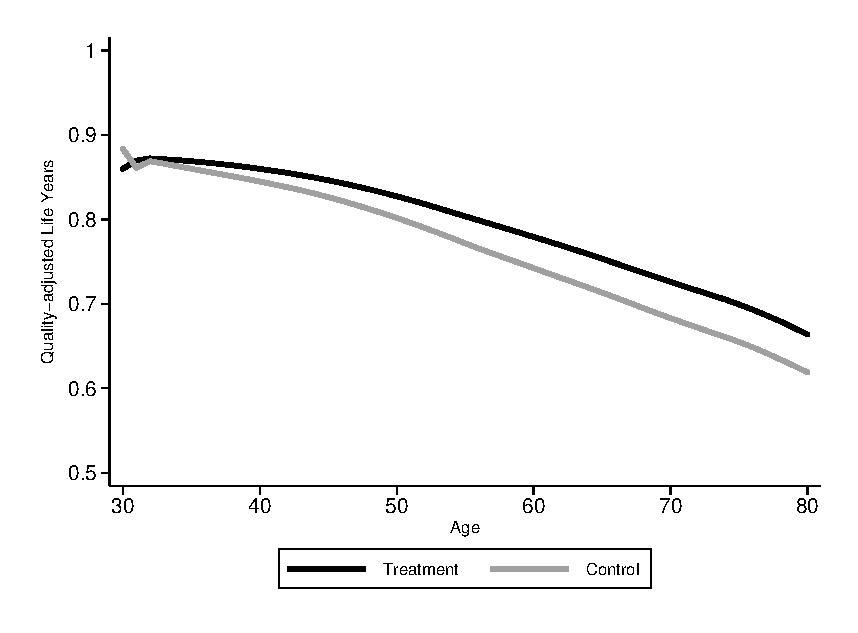
\includegraphics[height=3.5in]{AppOutput/Health/ABC-FAM_qaly_surv_summary_male}
\end{subfigure}

\begin{subfigure}{.8\textwidth} %
  \centering
  \subcaption{Females}
  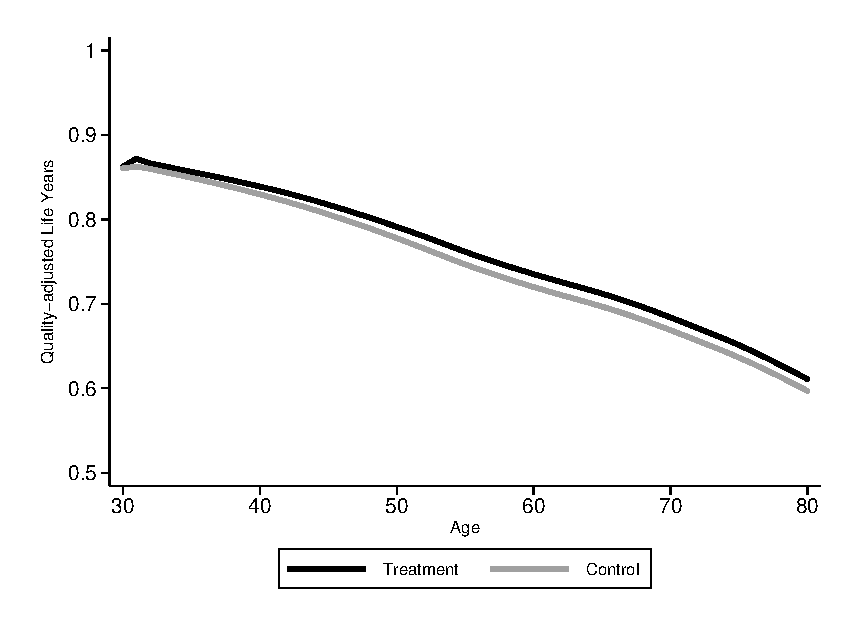
\includegraphics[height=3.5in]{AppOutput/Health/ABC-FAM_qaly_surv_summary_female}
\end{subfigure}
\floatfoot{
\footnotesize
\noindent Note: Panel (a) displays the predicted Quality-Adjusted Life Years (QALYs) from age 30 for males, conditional on survival. Panel (b) displays the predicted Quality-Adjusted Life Years (QALYs) from age 30 for females, conditional on survival.
}
\end{figure}
\begin{figure}[H]
    \centering
\caption{Predicted Total Medical Costs} \label{figure:totmd}
\begin{subfigure}{.8\textwidth}
  \centering
  \subcaption{Males}
  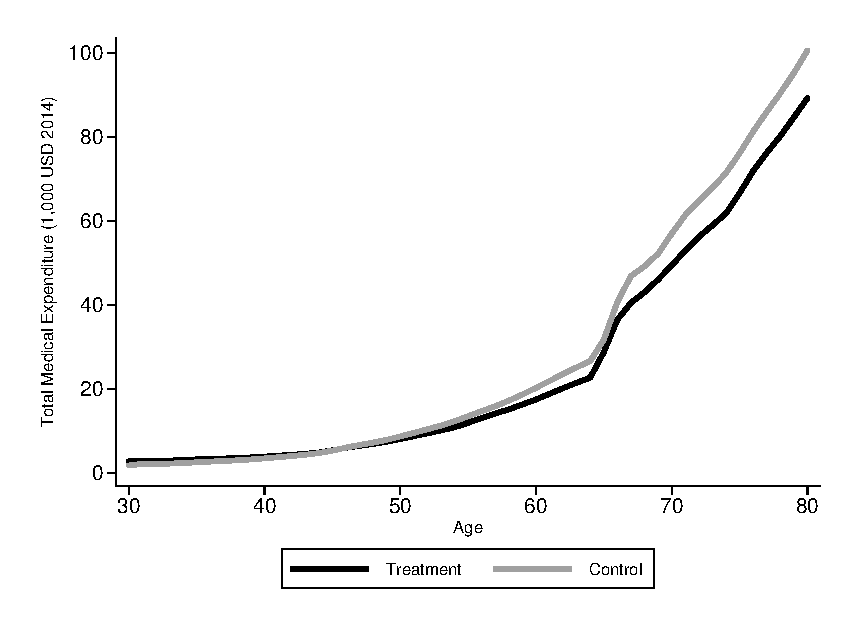
\includegraphics[height=3.5in]{AppOutput/Health/ABC-FAM_totmd_surv_summary_male}
\end{subfigure}

\begin{subfigure}{.8\textwidth} %
  \centering
  \subcaption{Females}
  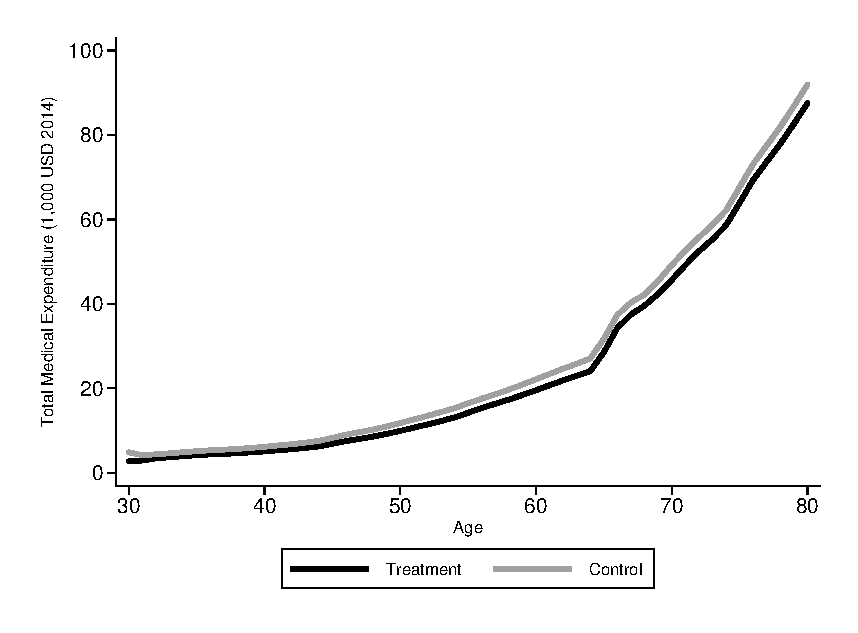
\includegraphics[height=3.5in]{AppOutput/Health/ABC-FAM_totmd_surv_summary_female}
\end{subfigure}
\floatfoot{
\footnotesize
\noindent Note: Panel (a) displays the predicted total medical costs for males over the life cycle from age 30 in 2009 USD, conditional on survival. Panel (b) displays the predicted total medical costs for females over the life-cycle from age 30 in 2009 USD, conditional on survival.
}
\end{figure}

\noindent Figure~\ref{figure:qaly} shows that predicted QALYs are higher over the entire life cycle for the treatment group than for the control group. This difference appears to be larger for males. This is not surprising, given that males show larger treatment effects in prevalence rates of disease than do females. Similarly, projected total medical costs are lower for the treatment group than for the control group over the entire life-cycle, as shown in Figure~\ref{figure:totmd}.
Figure~\ref{figure:fam_survival} shows estimates of the survival probability for the treatment and control groups in FAM. There is a substantial difference in survival rates in favor of males in the treatment groups when compared with those in the control groups. \\


\begin{figure}[H]
    \centering
\caption{Predicted Survival} \label{figure:fam_survival}
\begin{subfigure}{.8\textwidth}
  \centering
  \subcaption{Males}
  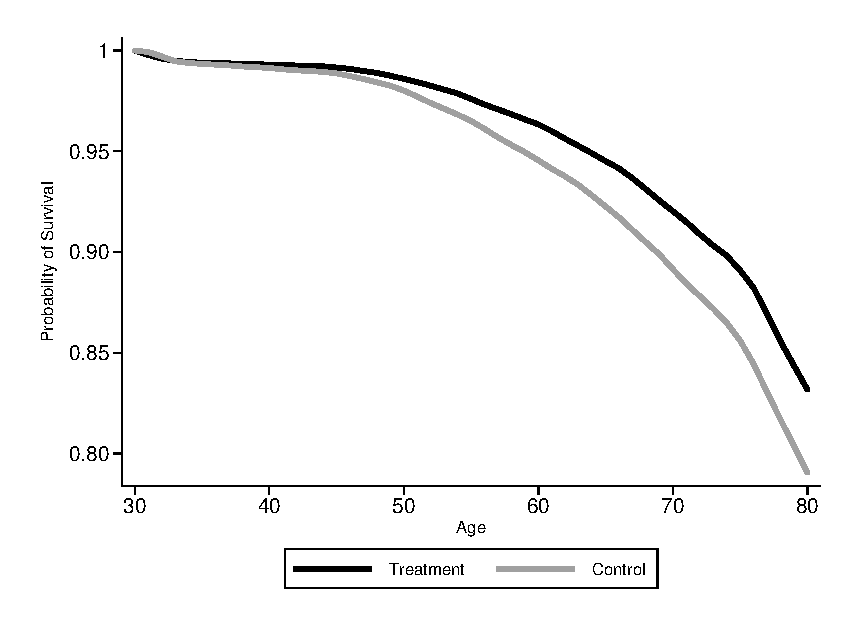
\includegraphics[height=3.5in]{AppOutput/Health/ABC-FAM_survival_male}
\end{subfigure}

\begin{subfigure}{.8\textwidth} %
  \centering
  \subcaption{Females}
  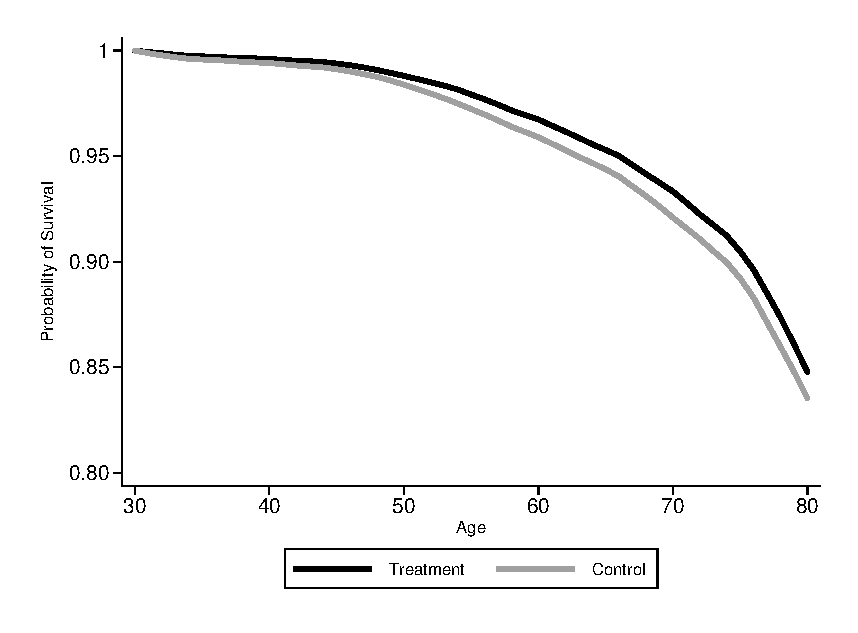
\includegraphics[height=3.5in]{AppOutput/Health/ABC-FAM_survival_female}
\end{subfigure}
\floatfoot{
\footnotesize
\noindent Note 1 Panel (a) displays the predicted survival for males after age-30 interview. Panel (b) displays the predicted survival for females after age-30 interview. Individual-level survival probabilities are calculated by estimating age-specific mortality probabilities for each subject using the FAM simulation results.  The individual-level survival probabilities are then averaged over the number of subjects in each group who had completed the age 34 interview.
}
\end{figure}

\noindent To quantify the impact of treatment on health outcomes, for each simulated cohort, we compute the present discounted value of the difference between treatment and control in the average value of QALYs and average medical costs. We do this for every age. We assume a discount rate of 4\% for this analysis, and we include outcome averages from the start of the simulation at age 30 until death for each cohort. We follow the recent literature on benefit-cost analysis of medical interventions and value a QALY of 1 to be worth \$150,000.\footnote{For a discussion on the limitations of a single value per QALY, see \citet{Pinto-Prades_etal_2009_Trying-to-Estimate} and \citet{Mason_etal_2009_Modelling}. \citet{Grosse_2008_Assessing-Cost-Effectiveness} summarizes the history of QALY valuation.} The raw difference in present discounted value at birth between treatment and control groups amounts to $ \$37,316  $ (2014 USD) per individual. Accounting for attrition, this difference falls to $ \$19,985 $. Table~\ref{table:PDV} shows the present discounted value of health outcomes for treatment and control cohorts in the top panel. The bottom panel of Table~\ref{table:PDV} decomposes the treatment effects on health by gender. The difference in health by treatment group is larger for males than for females. To account for a lack of consensus on QALY valuation, we also present the results for a lower valuation of QALYs, following \citet{Cutler_Meara_1998_Med-Costs_BOOK}, in the second row of each panel of Table~\ref{table:PDV}.\footnote{In Appendix \ref{appendix:sensitivity}, we show how the internal rate of return and benefit-cost ratios are impacted by a range of valuations for QALYs.} In this case of lower valuation of QALYs, there is still a positive difference in net health outcomes in favor of the treatment groups over the control groups of $ \$26,374$. Accounting for attrition, this difference falls to $ \$13,323$. \\

\begin{table}[H]
\begin{threeparttable}
%\footnotesize
\small
\caption{Present Discounted Value of Health Net of Medical Costs, by Treatment Status} \label{table:PDV}
\begin{tabular}{ccccccc}
\hline \hline
QALY Valuation &  \multicolumn{2}{c}{Treatment}   & \multicolumn{2}{c}{Control} & \multicolumn{2}{c}{Treatment Effect}  \\ \hline

QALY valued \$150,000 &	\multicolumn{2}{c}{\$817,505  }	& \multicolumn{2}{c}{ \$780,189  } & \multicolumn{2}{c}{\$37,316 } \\ 
QALY valued \$100,000 & \multicolumn{2}{c}{ \$513,615   } & \multicolumn{2}{c}{\$487,241 }	&	\multicolumn{2}{c}{\$26,374 } \\ \hline 
&&&&&& \\
& Females & Males & Females & Males & Females & Males \\ \hline
QALY valued \$150,000 & \$806,622 	& \$828,387 	& \$777,446 	& \$787,732 	& \$29,177 	& \$40,655  \\
QALY valued \$100,000 & \$504,058 	& \$523,172 	& \$483,063 	& \$498,731 	& \$20,995 	& \$24,441  \\ 
\hline \hline 
\end{tabular}

\begin{tablenotes}
\footnotesize
\item Note: This table summarizes the present discounted value at birth, at a 4\% annual discount rate in 2014 USD, of the health outcomes measured through QALYs, net of medical costs, from age 30 until death. \\
\end{tablenotes}
\end{threeparttable}
\end{table}


